% This must be in the first 5 lines to tell arXiv to use pdfLaTeX, which is strongly recommended.
\pdfoutput=1
% In particular, the hyperref package requires pdfLaTeX in order to break URLs across lines.

\documentclass[11pt]{article}

% Remove the "review" option to generate the final version.
% \usepackage{ACL2023}
\usepackage[review]{ACL2023}

% Standard package includes
\usepackage{times}
\usepackage{latexsym}

% For proper rendering and hyphenation of words containing Latin characters (including in bib files)
\usepackage[T1]{fontenc}
% For Vietnamese characters
% \usepackage[T5]{fontenc}
% See https://www.latex-project.org/help/documentation/encguide.pdf for other character sets

% This assumes your files are encoded as UTF8
\usepackage[utf8]{inputenc}

% This is not strictly necessary, and may be commented out.
% However, it will improve the layout of the manuscript,
% and will typically save some space.
\usepackage{microtype}

% This is also not strictly necessary, and may be commented out.
% However, it will improve the aesthetics of text in
% the typewriter font.
\usepackage{inconsolata}

% Manually added
\usepackage{float}
\usepackage{amsmath}
\usepackage{amssymb}
\usepackage{hyperref}
\usepackage{graphicx}
\usepackage{algorithm}
\usepackage{algpseudocode}

\renewcommand{\sectionautorefname}{Section}

\makeatletter
\@ifpackagewith{ACL2023}{review}{
    % Code if "review" option is enabled
    \newcommand{\noreview}[1]{}
}{
    % Code if "review" option is NOT enabled
    \newcommand{\noreview}[1]{#1}
}
\makeatother

% If the title and author information does not fit in the area allocated, uncomment the following
%
%\setlength\titlebox{<dim>}
%
% and set <dim> to something 5cm or larger.

\title{Automatic Summarization of Long Documents}

% Author information can be set in various styles:
% For several authors from the same institution:
% \author{Author 1 \and ... \and Author n \\
%         Address line \\ ... \\ Address line}
% if the names do not fit well on one line use
%         Author 1 \\ {\bf Author 2} \\ ... \\ {\bf Author n} \\
% For authors from different institutions:
% \author{Author 1 \\ Address line \\  ... \\ Address line
%         \And  ... \And
%         Author n \\ Address line \\ ... \\ Address line}
% To start a seperate ``row'' of authors use \AND, as in
% \author{Author 1 \\ Address line \\  ... \\ Address line
%         \AND
%         Author 2 \\ Address line \\ ... \\ Address line \And
%         Author 3 \\ Address line \\ ... \\ Address line}

\author{
	Naman Chhibbar \\
	IIT Hyderabad \\
	Kandi, Sangareddy \\
	Telangana 502285, India \\
	\texttt{ma21btech11011@iith.ac.in}
	\And
	Jugal Kalita \\
	University of Colorado, Colorado Springs \\
	1420 Austin Bluffs Pkwy \\
	Colorado Springs CO 80918 \\
	\texttt{jkalita@uccs.edu}
}

\begin{document}
	\maketitle

	\begin{abstract}

A vast amount of text is added to the internet daily, making utilization and interpretation of textual data complex and cumbersome.
As a result, automatic text summarization is crucial for extracting relevant information, saving precious time.
Although many transformer models excel in summarization, they are constrained by their input size, preventing them from processing texts longer than their context size.
This study introduces three novel algorithms that allow any LLM to efficiently overcome its input size limitation, effectively utilizing its full potential without any architectural modifications.
We test our algorithms on texts with more than 70,000 words, and our experiments show a significant increase in BERTScore with competitive ROUGE scores.

\end{abstract}

	\section{Introduction}
\label{sec:introduction}

Due to the ever-increasing amount of textual data available online, document summarization has become crucial for the efficient and accurate extraction of relevant information.
Large Language Models (LLMs) based on the transformer architecture \cite{vaswani2017attention} have shown outstanding abilities in many NLP tasks, including document summarization \cite{yadav2023state}.
Recent developments have demonstrated remarkable improvements in the relevancy and coherence of summaries generated by such LLMs.

However, long document summarization, which involves removing redundancies and makes reading long texts concise and efficient, remains a major challenge.
One of the significant limitations in the transformer architecture is limited context size, stemming from the quadratic memory and computational complexity of the attention mechanism \cite{du2023improving}.
This constraint hinders extracting relevant information from extensive texts where summarization is valuable to overcome the time, effort, and interpretive issues posed by complex and large documents.

We experiment with three novel approaches to address the input size limitations of transformers.
The methods introduced do not include any architectural modifications to the model used and can be incorporated into any existing pipeline.
We believe that these methods can effectively utilize the full potential of any existing LLM by capturing information from crucial aspects of the document.
Though our experiments only include the task of summarization, we hypothesize that our methods can be applied to NLP tasks that require processing long texts.

We start by stating the problem statement (\autoref{sec:problem}) and discussing related works (\autoref{sec:related-works}) to gain insights into the problem and the state-of-the-art solutions.
We then introduce the datasets (\autoref{sec:datasets}) and methodology (\autoref{sec:methodology}) used in our experiments.
For evaluating our results, we present some standard metrics (\autoref{sec:metrics}) used in text summarization.
We end the report by discussing our experimental findings (\autoref{sec:findings}) and potential future work (\autoref{sec:future-work}) and concluding the study (\autoref{sec:conclusion}).

	\section{Problem Statement}


\begin{frame}{The Problem}

\begin{itemize}
	\item LLMs suffer from one major limitation: limited context size.
	\item<2-> This is due to the quadratic self-attention mechanism in the transformer
	architecture.
	\item<3-> For example, BERT has a context size of just 512 tokens (about half page
	of text).
	\item<4> Due to this, LLMs can not process long texts wherein summarization is
	valuable for efficient extraction of information.
\end{itemize}

\end{frame}

	\section{Related Works}

In this section, we discuss some recent works related to long document summarization.


\subsection*{Longformer}

\citet{beltagy2020longformer} introduce Longformer, a tranformer modified to handle
long sequences.
They do this by replacing the quadratic self attention mechanism in the transformer
architecture with a sliding window self attention, which has a linear complexity
with respect to input size.
To capture global dependencies, they add global attention to pre-selected input
positions.
They have also experimented with dilated sliding window and ablated models.


\subsection*{Summarization of Long Meeting Transcripts}

\citet{10.1145/3639233.3639253} describe a unique way of summarizing long meeting
transcripts.
Their approach is based on "Divide-and-Conquer", which starts with
segmenting the transcript to summarize each segment individually and combine them.
They use the BART (Bidirectional and Auto-Regressive Transformer) model to summarize
the segments due to its high speed and performance.
They also extract action-item pairs to aid summarization.
After processing every segment, all summaries are combined for a final abstractive
summarization.
If the combined summary fails to fit the context size, the combined summary is
recursively segmented and summarized again.
This study gives us insights into how we can process long inputs for summarization.


\subsection*{Question-Answering on Long Videos}

\citet{wang2024videoagent} introduce VideoAgent, an AI agent designed to answer a
given question using the context of a long video (approximately an hour long).
The agent first generates captions from multiple uniformly sampled frames from the
video, which are used to answer the question.
If the agent feels that the captions are not sufficient to answer the question, it
identifies a segment between the initial frames to obtain more frames.
This work is relevant since a long video, a sequence of frames, can be considered
analogous to a long document, a sequence of tokens. The techniques utilized by
VideoAgent can be adapted to perform query-based summarization in long documents.


\subsection*{Long Chinese News Classification}

\citet{chen2022long} describe a novel algorithm for long document classification
aimed to classify Chinese news into a set of pre-defined categories.
Their approach begins with pre-processing a long text by segmenting it into sentences
and forming groups of sentences determined by a fixed maximum number of tokens a
group should have.
BERT is then used to encode these groups of sentences for further processing.
Each sentence embedding is passed through a 1D convolution layer for local feature
extraction, followed by a 1D max-pooling layer.
Finally, a classifier head with softmax activation is used to classify using the
extracted features.
Methods utilized in this video, like segmenting and convolving, may prove helpful in
encoding long documents.

	\section{Datasets}


\subsection*{GovReport}

Introduced by \citet{huang-etal-2021-efficient}, this dataset consists of
reports written by government research agencies, including the Congressional
Research Service and the U.S. Government Accountability Office.
Texts and summaries have an average word count of 7,700.71 and 451.36,
respectively, with a max word count of 73,815 and 1,442.
Figure \ref{fig:govreport} shows the word count distribution of the dataset.

\begin{figure}[!ht]
	\centering
	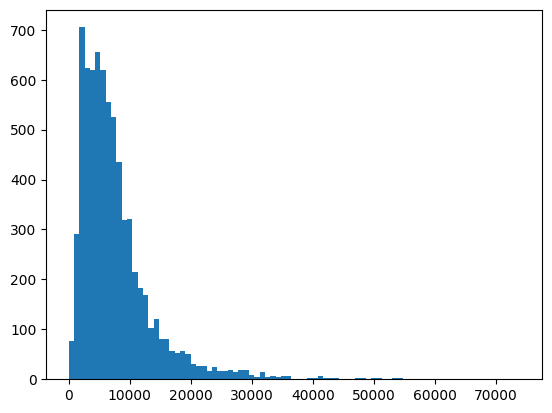
\includegraphics[width=.48\textwidth]{Images/govreport-wordcount.jpg}
	\caption{GovReport word counts}
	\label{fig:govreport}
\end{figure}


\subsection*{BigPatent}

Not used yet. \nocite{sharma-etal-2019-bigpatent}

	\section{Methodology}
\label{sec:methodology}

We discuss the methodology used in our experiments in this section.
Most of the methods start by segmenting the document into smaller, contiguous, and
exhaustive parts.
The segmentation algorithm is controlled by a threshold on the minimum number of words
in a segment, which is a hyperparameter in each of the respective methods.


\subsection{Central Truncation}
\label{method:truncation}

Truncation is the most common and straightforward approach used to handle long texts
that exceed the context size of an LLM.
It is done in three main ways:

\begin{itemize}
	\item \textbf{Retaining Head}: Keeping tokens from the start.
	\item \textbf{Retaining Tail}: Keeping tokens from the end.
	\item \textbf{Head and Tail}: Keeping tokens from both start and end.
\end{itemize}

\citet{worsham-kalita-2018-genre} also employ "retaining head" and "retaining tail"
strategies on long texts and find promising results.
Though the "retaining head" method is often used, keeping the initial tokens allowed
by the LLM, \citet{sun2019fine} have found that keeping both head and tail produces
better results than both the "retaining head" and the "retaining tail" methods.
Their research also shows that truncating the middle is even better than the more
complicated hierarchical methods, displaying superiority with simplicity.

The fraction of tokens to be taken from the head is controlled by the hyperparameter
$head\_size \in [0, 1]$.
Setting $head\_size = 1$ results in taking tokens only from the head, whereas
setting $head\_size = 0$ results in taking tokens only from the tail.
The truncated text is then sent to the summarizer.


\subsection{Document Skimming}
\label{method:skimming}

One way to process long texts is by employing a speed reading strategy known as "skimming".
Skimming is done by reading the whole text in a go while selectively skipping some
parts of the text for quicker reading.
The reader usually omits the portions that seem redundant or irrelevant in the text,
minimizing information loss.

This method starts by segmenting the text using a segmenter with the hyperparameter $min\_words$.
The segmenter uses a sentence tokenizer to separate sentences from the text, and then
merges the sentences which have fewer words than $min\_words$.
We then sample segments uniformly, with each segment having probability $p$ to be picked.
The sampled segments are then merged to form a single text and sent to the summarizer.
This ensures we sample a segment from each part of the text.

To address the removal of redundancy in the document, we experiment with and without removing
redundant segments before and after sampling.
This is done by computing the cosine similarity between the mean segment embeddings and the current
segment embedding.
\href{https://huggingface.co/sentence-transformers/all-MiniLM-L6-v2}{This} sentence transformer
is used to generate the segment embeddings.
This sentence transformer is based on MiniLM \cite{wang2020minilm}, which is a distilled version
of larger encoder-only transformer models.
If the cosine similarity is greater than a threshold, the current segment is removed.
The mean embedding is updated if the current segment is retained.

When removing segments after sampling, we increase the probability of choosing the segments
before sampling to compensate for the removed segments.
This fraction is controlled by the hyperparameter $prob\_boost$.
The updated probability is calculated as $p_{new} = (1 + prob\_boost) \cdot p_{optimal}$.
Though removing redundant segments before sampling is less efficient due to the whole document
being processed, it ensures better utilization of the LLM's context size.
The mean embedding is initialised as a zero vector and updated after each segment is processed.
Doing so introduces a hyperparameter $threshold$ to control the similarity threshold between the
mean embedding and the current segment embedding.

This approch is a modification to the methodology \citet{wang2024videoagent} use for
question-answering on long videos. \citet{worsham-kalita-2018-genre} also use random sampling
for genre identification.

We will now discuss the calculation of the optimal value of $p$ here.
Let $X$ denote the total number of tokens in the sampled segments.
Since segments are sampled randomly, $X$ is a random variable.
If the context size of the model is $model\_size$, we want $\mathrm{E}[X] = model\_size$,
where $\mathrm{E}[X]$ denotes the expectation of $X$.

Suppose we have $n \in \mathbb{N}$ segments and $X_i \sim \mathrm{Bernoulli}(p)$ denotes
if segment $i$ is chosen, $i \in \{1, 2, \dots, n\}$.
If $len_i$ denotes the number of tokens in segment $i$, we can write:

\[ X = \sum_{i = 1}^{n} X_i \cdot len_i \]
\[ \Rightarrow \mathrm{E}[X] = \mathrm{E}[\sum_{i = 1}^{n} X_i \cdot len_i] \]
\[ \Rightarrow \mathrm{E}[X] = \sum_{i = 1}^{n} \mathrm{E}[X_i \cdot len_i] \]
\[ \Rightarrow \mathrm{E}[X] = \sum_{i = 1}^{n} \mathrm{E}[X_i] \cdot len_i \]

Since $X_i \sim \mathrm{Bernoulli}(p)$ $\forall i \in \{1, 2, \dots, n\}$, we
have $\mathrm{E}[X_i] = p$ $\forall i \in \{1, 2, \dots, n\}$.

\[ \Rightarrow \mathrm{E}[X] = \sum_{i = 1}^{n} p \cdot len_i \]
\[ \Rightarrow \mathrm{E}[X] = p \cdot \sum_{i = 1}^{n} len_i \]

Let $total\_len$ be the total number of tokens in the text, then
$total\_len = \sum_{i = 1}^{n} len_i$.

\[ \therefore \mathrm{E}[X] = p \cdot total\_len = model\_size \]
\[ \Rightarrow p \cdot total\_len = model\_size \]
\[ \therefore p = model\_size / total\_len \]


\subsection{Document Skimming with Keyword Extraction}
\label{method:skimming-keyword}

Document skimming (\ref{method:skimming}) involved a very intuitive and simple
approach of sampling segments randomly.
Instead of that, we can use an efficient keyword extraction algorithm to get important keywords
from the document.
These keywords help us sample segments intelligently, ensuring we get the most important
segments from the document.

We use Latent Dirichlet Allocation (LDA) \cite{blei2003latent} with a single topic to get topic
words (keywords) from the document.
These keywords are concatenated using a delimiter (a space is used in our experiments) to form a
single sentence.
This sentence is then embedded and compared with other segment embeddings using cosine similarity.
Maximum number of segments with the highest similarity are retained.
The keyword sentence and document segments are embedded using the same
\href{https://huggingface.co/sentence-transformers/all-MiniLM-L6-v2}{sentence transformer}
used in the previous method.

This approach is similar to the way \citet{golia2024action} use action items to pick segments of
text (a neighbourhood of 2 sentences around the action item) for summarization.


% \subsection{Summarization using Convolutions}

% Another way to approach the problem is to apply convolution to encoded segments of
% the document.
% The convolution operation multiplies a sliding window of weights element-wise by the
% embeddings and then sums the result.
% This allows the model to learn cross-segment relationships and acts as a
% limited-range attention mechanism, an algorithm similar to \citet{chen2022long}.

% This method begins with separating sentences from the document and grouping them
% based on a fixed maximum number of sentences per group.
% These groups are then encoded and passed through a 1D convolution layer of size $k$ with
% $f$ filters, where $k$ and $f$ are hyperparameters in the model.
% A max-pooling layer can also be applied for feature enhancement.
% A decoder-only transformer then uses these processed embeddings as keys and values
% for the encoder-decoder attention mechanism to generate the summary.

% Longformer model \cite{beltagy2020longformer} uses a windowed attention mechanism with
% linear complexity to process long texts.
% Our 1D convolution operation outperforms the windowed attention mechanism since it has
% linear complexity and is more efficient to calculate than attention.

	\section{Evaluation Metrics}
\label{sec:metrics}

The best way to evaluate generated natural language is by humans, but conducting human trials is expensive and time-consuming.
Due to this difficulty, we use automatic evaluation metrics to evaluate the quality of the generated summary given some reference summaries.
\citet{fabbri2021summeval} review many such open-source and state-of-the-art metrics.
The two that we use in our experiments are discussed below.
These metrics are commonly used in published literature.

\textbf{ROUGE metrics:} \citet{lin-2004-rouge} introduces the Recall-Oriented Understudy for Gisting Evaluation (ROUGE) metrics.
The basic ROUGE-N metric is based on the fraction of overlaps of ideal or reference summaries with the candidate summary, hence being recall-oriented.
His study concludes that ROUGE-N with $\text{N} = 2$, ROUGE-L, ROUGE-W, and ROUGE-S work well for the summarization task.

\textbf{BERTScore:} \citet{zhang2019bertscore} introduce BERTScore, an automatic evaluation metric for text generation.
BERTScore is calculated by comparing the contextual embeddings of tokens in the candidate and reference summaries, which are generated using BERT \cite{devlin2018bert}.
BERTScore excels at capturing semantic similarities between sentences since it uses contextual embeddings of tokens instead of N-gram frequencies to calculate similarity.

	\section{Experimental Findings}
	\label{sec:findings}


	\begin{table*}[!ht]
		\centering

		\begin{tabular}{c c c c c}
			\hline
			Model & ROUGE-1 & ROUGE-2 & ROUGE-L & BERTScore \\
			\hline
			BART w/ Unlimiformer (1,024) & 53.4 & 22.5 & 22.5 & 66.0 \\
			PRIMERA w/ Unlimiformer (4,096) & 56.5 & 24.8 & 26.3 & 67.7 \\
			Hepos (10,240) & 51.34 & 19.09 & \textbf{48.73} & - \\
			PEGASUS-X w/ Staggered & 60.3 & \textbf{30.0} & 31.5 & - \\
			Block-Local Attention (16k) & & & & \\
			LLaMA-7B w/ Positional & 60.0 & 28.0 & 29.5 & - \\
			Interpolation (15k) & & & & \\
			\hline
			Summarization w/ Extraction & \textbf{61.99} & 18.52 & 38.46 & \textbf{86.20} \\
			+ GPT-3.5 Turbo (4,096) & & & & \\
			Central truncation + LongT5 (4,096) & 46.20 & 4.38 & 38.27 & \textbf{82.19} \\
			Skimming w/ post-sampling & 46.76 & 4.56 & 39.61 & \textbf{81.96} \\
			removal + LongT5 (4,096) & & & & \\
			\hline
		\end{tabular}

		\caption{Automatic evaluation results on the GovReport dataset. Context size of the models are
		mentioned in parentheses. The best score in each metric category is highlighted in \textbf{bold}.}
		\label{tab:govreport}
	\end{table*}

	\begin{table*}[!ht]
		\centering

		\begin{tabular}{c c c c c}
			\hline
			Model & ROUGE-1 & ROUGE-2 & ROUGE-L & BERTScore \\
			\hline
			BigBird-Pegasus (16k) & \textbf{60.64} & \textbf{42.46} & \textbf{50.01} & - \\
			\hline
			Skimming w/ pre-sampling & 27.40 & 3.31 & 21.25 & \textbf{82.62} \\
			removal + GPT-3.5 Turbo (4,096) & & & & \\
			Central truncation + GPT-3.5 Turbo (4,096) & 27.77 & 3.09 & 20.56 & \textbf{82.57} \\
			Skimming w/ post-sampling & 26.16 & 2.13 & 20.21 & \textbf{82.40} \\
			removal + GPT-3.5 Turbo (4,096) & & & & \\
			\hline
		\end{tabular}

		\caption{Automatic evaluation results on the BigPatent dataset. Context size of the models are
		mentioned in parentheses. The best score in each metric category is highlighted in \textbf{bold}.}
		\label{tab:bigpatent}
	\end{table*}

	We test our pipelines with the following models: \textbf{BART} (Bidirectional
	and Autoregressive Transformer) \cite{lewis-etal-2020-bart} fine-tuned on the
	CNN/Daily Mail dataset \cite{nallapati2016abstractive} with a context size of 1024,
	\textbf{LongT5} \cite{guo2021longt5}, a variant of T5 (Text-to-Text Transfer
	Transformer) \cite{raffel2020exploring}, fine-tuned on the BookSum dataset with
	a context size of 4096, and \textbf{GPT-3.5 Turbo} \cite{brown2020language} with a
	context size of 4096.

	We compare our results with the state-of-the-art summarization models on the GovReport dataset,
	including Unlimiformer \cite{bertsch2023unlimiformer} integrated with BART
	\cite{lewis-etal-2020-bart} and PRIMERA \cite{beltagy2020longformer}, Hepos
	\cite{huang-etal-2021-efficient}, PEGASUS-X with staggered block-local attention
	\cite{phang2022investigating}, extended	LLaMA-7B with positional interpolation
	\cite{chen2023extending}.
	We also compare our results with BigBird-Pegasus \cite{zaheer2020big} on the BigPatent dataset.
	Refer to \autoref{tab:govreport} and \autoref{tab:bigpatent} for results on the GovReport and 
	BigPatent datasets, respectively.

	We were unable to confirm the BERTScores of our baselines, except for Unlimiformer, due to
	unavailability of code or computational limitations.


	\subsection*{Time complexity analysis}

		We evaluate the time complexity of our methods by measuring the mean time taken to process a
		document (excluding the time taken by the model to generate the summaries).
		We find that Central Truncation (\ref{method:truncation}) and Document Skimming
		(\ref{method:skimming}) take approximately the same time.
		Skimming with post-sampling removal takes slightly more time than the other two methods.
		We can see a significant increase in time taken by Skimming with pre-sampling removal
		and Summarization with Keyword Extraction (\ref{method:keyword}) due to the additional
		computations required.
		\autoref{fig:times} illustrates the average time taken by our methods.
		Check \autoref{tab:encoder-times} for exact values rounded off to two decimal places.

		\begin{figure}[!ht]
			\centering
			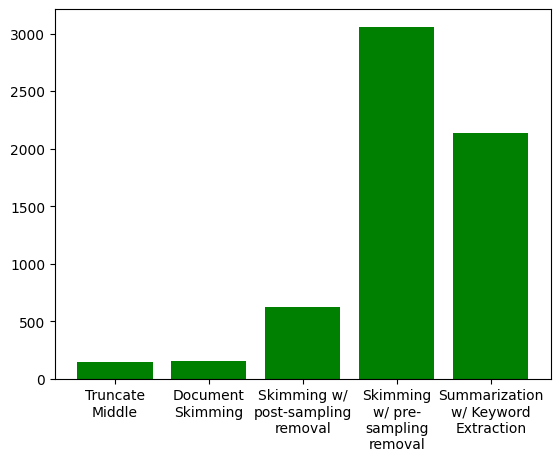
\includegraphics[width=.48\textwidth]{Images/encoder-times.png}
			\caption{Mean time taken per document using BART tokenizer on BigPatent dataset}
			\label{fig:times}
		\end{figure}

		\begin{table}[!ht]
			\centering

			\begin{tabular}{c c}
				\hline
				Method & Mean time taken \\
				\hline
				Central Truncation & 142.50 ms \\
				Document Skimming & 155.42 ms \\
				Skimming w/ post- & 625.17 ms \\
				sampling removal & \\
				Skimming w/ pre- & 3059.63 ms \\
				sampling removal & \\
				Summarization & 2131.40 ms \\
				w/ Extraction & \\
				\hline
			\end{tabular}

			\caption{Mean time taken per document using BART tokenizer on BigPatent dataset}
			\label{tab:encoder-times}
		\end{table}

	\section{Future Work}
\label{sec:future-work}

We have used a very basic sentence tokenizer
(\href{https://www.nltk.org/api/nltk.tokenize.sent_tokenize.html}{nltk.sent\_tokenize}),
with some modifications to control the minimum number of words in a segment,
to segment the document.
In our experiments, we find that segmentation is a crucial step in the pipeline, and can
influence the output summary significantly.
Ensuring the uniformity of the length of the segments while preserving coherence is
important for better utilization of the context size of the summarizer while sampling.
We encourage future work to experiment with more complex segmenters.

Future work can also be focused on extending the Summarization with Keyword Extraction
(\ref{method:keyword}) method.
Experimenting with different keyword extraction algorithms and use cases is encouraged.


\section{Conclusion}
\label{sec:conclusion}

Our experiments show that Document Skimming with post-sampling removal
(\ref{method:skimming}) performs well while being efficient.
The Central Truncation method (\ref{method:truncation}) also show good results,
which shows that simple methods can also be effective in long document summarization.
The last two methods, Skimming with pre-sampling removal and Summarization with Keyword
Extraction (\ref{method:keyword}), show the best results but are computationally expensive.

Our experiments show a huge jump in BERTScore compared to Unlimiformer on documents
with word counts upto 70,000.
This shows that our pipelines are able utilize details in long texts efficiently.
Even though our ROUGE-2 scores are lower than the baselines, ROUGE-1 and ROUGE-L
scores are competitive.
Since BERTScore is a better metric for capturing semantic similarity, we hypothesize
our pipelines are able to generate better summaries than the baselines with higher
ROUGE scores.


\section*{Acknowledgement}

All work herein reported is supported by the Nation Science Foundation under Grant
No. 2349452.

Any opinion, finding, or conclusion in this study is that of the authors and does not
necessarily reflect the views of the National Science Foundation.


	\bibliography{anthology}
	\bibliographystyle{acl_natbib}

\end{document}
